\documentclass[journal]{IEEEtran}
% If IEEEtran.cls has not been installed into the LaTeX system files,
% manually specify the path to it like:
% \documentclass[journal]{../sty/IEEEtran}

% Import setup file with includes
% TODO: Set up figure references (using \ref{})
% Some very useful LaTeX packages include:
% (uncomment the ones you want to load)

%%%%%%%%%%%%%%%%%%%%%%%%%%%%%%%%%%%%%
% ***** Misc Utility Packages ***** %
%%%%%%%%%%%%%%%%%%%%%%%%%%%%%%%%%%%%%

%\usepackage{ifpdf}
% Heiko Oberdiek's ifpdf.sty is very useful if you need conditional
% compilation based on whether the output is pdf or dvi.
% usage:
% \ifpdf
%   % pdf code
% \else
%   % dvi code
% \fi
% The latest version of ifpdf.sty can be obtained from:
% http://www.ctan.org/pkg/ifpdf
% Also, note that IEEEtran.cls V1.7 and later provides a builtin
% \ifCLASSINFOpdf conditional that works the same way.
% When switching from latex to pdflatex and vice-versa, the compiler may
% have to be run twice to clear warning/error messages.

%%%%%%%%%%%%%%%%%%%%%%%%%%%%%%%%%
% ***** Citation Packages ***** %
%%%%%%%%%%%%%%%%%%%%%%%%%%%%%%%%%

\usepackage[
    style=ieee,
    backend=biber,
    sortcites=true,
    sorting=nyt,
%    isbn=false,
   url=true,
   doi=true,
%    eprint=false,
    hyperref=false,
    backref=false,
%    firstinits=false,
]{biblatex}
\usepackage{csquotes}

%\usepackage{cite}
% cite.sty was written by Donald Arseneau
% V1.6 and later of IEEEtran pre-defines the format of the cite.sty package
% \cite{} output to follow that of the IEEE. Loading the cite package will
% result in citation numbers being automatically sorted and properly
% "compressed/ranged". e.g., [1], [9], [2], [7], [5], [6] without using
% cite.sty will become [1], [2], [5]--[7], [9] using cite.sty. cite.sty's
% \cite will automatically add leading space, if needed. Use cite.sty's
% noadjust option (cite.sty V3.8 and later) if you want to turn this off
% such as if a citation ever needs to be enclosed in parenthesis.
% cite.sty is already installed on most LaTeX systems. Be sure and use
% version 5.0 (2009-03-20) and later if using hyperref.sty.
% The latest version can be obtained at:
% http://www.ctan.org/pkg/cite
% The documentation is contained in the cite.sty file itself.



%%%%%%%%%%%%%%%%%%%%%%%%%%%%%%%%%
% ***** Graphics Packages ***** %
%%%%%%%%%%%%%%%%%%%%%%%%%%%%%%%%%

\usepackage{graphicx}

\ifCLASSINFOpdf
  % \usepackage[pdftex]{graphicx}
  % declare the path(s) where your graphic files are
  % \graphicspath{{../pdf/}{../jpeg/}}
  % and their extensions so you won't have to specify these with
  % every instance of \includegraphics
  % \DeclareGraphicsExtensions{.pdf,.jpeg,.png}
\else
  % or other class option (dvipsone, dvipdf, if not using dvips). graphicx
  % will default to the driver specified in the system graphics.cfg if no
  % driver is specified.
  % \usepackage[dvips]{graphicx}
  % declare the path(s) where your graphic files are
  % \graphicspath{{../eps/}}
  % and their extensions so you won't have to specify these with
  % every instance of \includegraphics
  % \DeclareGraphicsExtensions{.eps}
\fi
% graphicx was written by David Carlisle and Sebastian Rahtz. It is
% required if you want graphics, photos, etc. graphicx.sty is already
% installed on most LaTeX systems. The latest version and documentation
% can be obtained at: 
% http://www.ctan.org/pkg/graphicx
% Another good source of documentation is "Using Imported Graphics in
% LaTeX2e" by Keith Reckdahl which can be found at:
% http://www.ctan.org/pkg/epslatex
%
% latex, and pdflatex in dvi mode, support graphics in encapsulated
% postscript (.eps) format. pdflatex in pdf mode supports graphics
% in .pdf, .jpeg, .png and .mps (metapost) formats. Users should ensure
% that all non-photo figures use a vector format (.eps, .pdf, .mps) and
% not a bitmapped formats (.jpeg, .png). The IEEE frowns on bitmapped formats
% which can result in "jaggedy"/blurry rendering of lines and letters as
% well as large increases in file sizes.
%
% You can find documentation about the pdfTeX application at:
% http://www.tug.org/applications/pdftex

%%%%%%%%%%%%%%%%%%%%%%%%%%%%%
% ***** Math Packages ***** %
%%%%%%%%%%%%%%%%%%%%%%%%%%%%%

%\usepackage{amsmath}
% A popular package from the American Mathematical Society that provides
% many useful and powerful commands for dealing with mathematics.
%
% Note that the amsmath package sets \interdisplaylinepenalty to 10000
% thus preventing page breaks from occurring within multiline equations. Use:
%\interdisplaylinepenalty=2500
% after loading amsmath to restore such page breaks as IEEEtran.cls normally
% does. amsmath.sty is already installed on most LaTeX systems. The latest
% version and documentation can be obtained at:
% http://www.ctan.org/pkg/amsmath

%%%%%%%%%%%%%%%%%%%%%%%%%%%%%%%%%%%%%%%%%
% ***** Specialized List Packages ***** %
%%%%%%%%%%%%%%%%%%%%%%%%%%%%%%%%%%%%%%%%%

%\usepackage{algorithmic}
% algorithmic.sty was written by Peter Williams and Rogerio Brito.
% This package provides an algorithmic environment fo describing algorithms.
% You can use the algorithmic environment in-text or within a figure
% environment to provide for a floating algorithm. Do NOT use the algorithm
% floating environment provided by algorithm.sty (by the same authors) or
% algorithm2e.sty (by Christophe Fiorio) as the IEEE does not use dedicated
% algorithm float types and packages that provide these will not provide
% correct IEEE style captions. The latest version and documentation of
% algorithmic.sty can be obtained at:
% http://www.ctan.org/pkg/algorithms
% Also of interest may be the (relatively newer and more customizable)
% algorithmicx.sty package by Szasz Janos:
% http://www.ctan.org/pkg/algorithmicx

%%%%%%%%%%%%%%%%%%%%%%%%%%%%%%%%%%
% ***** Alignment Packages ***** %
%%%%%%%%%%%%%%%%%%%%%%%%%%%%%%%%%%

%\usepackage{array}
% Frank Mittelbach's and David Carlisle's array.sty patches and improves
% the standard LaTeX2e array and tabular environments to provide better
% appearance and additional user controls. As the default LaTeX2e table
% generation code is lacking to the point of almost being broken with
% respect to the quality of the end results, all users are strongly
% advised to use an enhanced (at the very least that provided by array.sty)
% set of table tools. array.sty is already installed on most systems. The
% latest version and documentation can be obtained at:
% http://www.ctan.org/pkg/array


% IEEEtran contains the IEEEeqnarray family of commands that can be used to
% generate multiline equations as well as matrices, tables, etc., of high
% quality.

%%%%%%%%%%%%%%%%%%%%%%%%%%%%%%%%%%
% ***** Subfigure Packages ***** %
%%%%%%%%%%%%%%%%%%%%%%%%%%%%%%%%%%

%\ifCLASSOPTIONcompsoc
%  \usepackage[caption=false,font=normalsize,labelfont=sf,textfont=sf]{subfig}
%\else
%  \usepackage[caption=false,font=footnotesize]{subfig}
%\fi
% subfig.sty, written by Steven Douglas Cochran, is the modern replacement
% for subfigure.sty, the latter of which is no longer maintained and is
% incompatible with some LaTeX packages including fixltx2e. However,
% subfig.sty requires and automatically loads Axel Sommerfeldt's caption.sty
% which will override IEEEtran.cls' handling of captions and this will result
% in non-IEEE style figure/table captions. To prevent this problem, be sure
% and invoke subfig.sty's "caption=false" package option (available since
% subfig.sty version 1.3, 2005/06/28) as this is will preserve IEEEtran.cls
% handling of captions.
% Note that the Computer Society format requires a larger sans serif font
% than the serif footnote size font used in traditional IEEE formatting
% and thus the need to invoke different subfig.sty package options depending
% on whether compsoc mode has been enabled.
%
% The latest version and documentation of subfig.sty can be obtained at:
% http://www.ctan.org/pkg/subfig

%%%%%%%%%%%%%%%%%%%%%%%%%%%%%%
% ***** Float Packages ***** %
%%%%%%%%%%%%%%%%%%%%%%%%%%%%%%

%\usepackage{fixltx2e}
% fixltx2e, the successor to the earlier fix2col.sty, was written by
% Frank Mittelbach and David Carlisle. This package corrects a few problems
% in the LaTeX2e kernel, the most notable of which is that in current
% LaTeX2e releases, the ordering of single and double column floats is not
% guaranteed to be preserved. Thus, an unpatched LaTeX2e can allow a
% single column figure to be placed prior to an earlier double column
% figure.
% Be aware that LaTeX2e kernels dated 2015 and later have fixltx2e.sty's
% corrections already built into the system in which case a warning will
% be issued if an attempt is made to load fixltx2e.sty as it is no longer
% needed.
% The latest version and documentation can be found at:
% http://www.ctan.org/pkg/fixltx2e


%\usepackage{stfloats}
% stfloats.sty was written by Sigitas Tolusis. This package gives LaTeX2e
% the ability to do double column floats at the bottom of the page as well
% as the top. (e.g., "\begin{figure*}[!b]" is not normally possible in
% LaTeX2e). It also provides a command:
%\fnbelowfloat
% to enable the placement of footnotes below bottom floats (the standard
% LaTeX2e kernel puts them above bottom floats). This is an invasive package
% which rewrites many portions of the LaTeX2e float routines. It may not work
% with other packages that modify the LaTeX2e float routines. The latest
% version and documentation can be obtained at:
% http://www.ctan.org/pkg/stfloats
% Do not use the stfloats baselinefloat ability as the IEEE does not allow
% \baselineskip to stretch. Authors submitting work to the IEEE should note
% that the IEEE rarely uses double column equations and that authors should try
% to avoid such use. Do not be tempted to use the cuted.sty or midfloat.sty
% packages (also by Sigitas Tolusis) as the IEEE does not format its papers in
% such ways.
% Do not attempt to use stfloats with fixltx2e as they are incompatible.
% Instead, use Morten Hogholm'a dblfloatfix which combines the features
% of both fixltx2e and stfloats:
%
% \usepackage{dblfloatfix}
% The latest version can be found at:
% http://www.ctan.org/pkg/dblfloatfix




%\ifCLASSOPTIONcaptionsoff
%  \usepackage[nomarkers]{endfloat}
% \let\MYoriglatexcaption\caption
% \renewcommand{\caption}[2][\relax]{\MYoriglatexcaption[#2]{#2}}
%\fi
% endfloat.sty was written by James Darrell McCauley, Jeff Goldberg and 
% Axel Sommerfeldt. This package may be useful when used in conjunction with 
% IEEEtran.cls'  captionsoff option. Some IEEE journals/societies require that
% submissions have lists of figures/tables at the end of the paper and that
% figures/tables without any captions are placed on a page by themselves at
% the end of the document. If needed, the draftcls IEEEtran class option or
% \CLASSINPUTbaselinestretch interface can be used to increase the line
% spacing as well. Be sure and use the nomarkers option of endfloat to
% prevent endfloat from "marking" where the figures would have been placed
% in the text. The two hack lines of code above are a slight modification of
% that suggested by in the endfloat docs (section 8.4.1) to ensure that
% the full captions always appear in the list of figures/tables - even if
% the user used the short optional argument of \caption[]{}.
% IEEE papers do not typically make use of \caption[]'s optional argument,
% so this should not be an issue. A similar trick can be used to disable
% captions of packages such as subfig.sty that lack options to turn off
% the subcaptions:
% For subfig.sty:
% \let\MYorigsubfloat\subfloat
% \renewcommand{\subfloat}[2][\relax]{\MYorigsubfloat[]{#2}}
% However, the above trick will not work if both optional arguments of
% the \subfloat command are used. Furthermore, there needs to be a
% description of each subfigure *somewhere* and endfloat does not add
% subfigure captions to its list of figures. Thus, the best approach is to
% avoid the use of subfigure captions (many IEEE journals avoid them anyway)
% and instead reference/explain all the subfigures within the main caption.
% The latest version of endfloat.sty and its documentation can obtained at:
% http://www.ctan.org/pkg/endfloat
%
% The IEEEtran \ifCLASSOPTIONcaptionsoff conditional can also be used
% later in the document, say, to conditionally put the References on a 
% page by themselves.

%%%%%%%%%%%%%%%%%%%%%%%%%%%%%%%%%%%%%%%%%%%%%%%
% ***** PDF, URL AND HYPERLINK PACKAGES ***** %
%%%%%%%%%%%%%%%%%%%%%%%%%%%%%%%%%%%%%%%%%%%%%%%

%\usepackage{url}
% url.sty was written by Donald Arseneau. It provides better support for
% handling and breaking URLs. url.sty is already installed on most LaTeX
% systems. The latest version and documentation can be obtained at:
% http://www.ctan.org/pkg/url
% Basically, \url{my_url_here}.




% *** Do not adjust lengths that control margins, column widths, etc. ***
% *** Do not use packages that alter fonts (such as pslatex).         ***
% There should be no need to do such things with IEEEtran.cls V1.6 and later.
% (Unless specifically asked to do so by the journal or conference you plan
% to submit to, of course. )


% correct bad hyphenation here
\hyphenation{op-tical net-works semi-conduc-tor}

%%%%%%%%%%%%%%%%%%%%%%%%%%%%%%%%%%%%%%%%%%
% ***** Code Listing Package Setup ***** %
%%%%%%%%%%%%%%%%%%%%%%%%%%%%%%%%%%%%%%%%%%

\usepackage{listings}
\usepackage{xcolor}
%New colors defined below
\definecolor{codegreen}{rgb}{0,0.6,0}
\definecolor{codegray}{rgb}{0.5,0.5,0.5}
\definecolor{codepurple}{rgb}{0.58,0,0.82}
\definecolor{backcolour}{rgb}{0.95,0.95,0.92}

%Code listing style named "mystyle"
\lstdefinestyle{mystyle}{
  backgroundcolor=\color{backcolour},   commentstyle=\color{codegreen},
  keywordstyle=\color{magenta},
  numberstyle=\tiny\color{codegray},
  stringstyle=\color{codepurple},
  basicstyle=\ttfamily\footnotesize,
  breakatwhitespace=false,         
  breaklines=true,                 
  captionpos=b,                    
  keepspaces=true,                 
  numbers=left,                    
  numbersep=5pt,                  
  showspaces=false,                
  showstringspaces=false,
  showtabs=false,                  
  tabsize=2
}

\lstset{style=mystyle}
\renewcommand{\lstlistingname}{Code Block}

\title{RBE 550 Homework 1 Documentation}

% TODO: Fix authors
\author{Alex Tacescu | Spring 2021
% <-this % stops a space
% \thanks{M. Shell was with the Department
% of Electrical and Computer Engineering, Georgia Institute of Technology, Atlanta,
% GA, 30332 USA e-mail: (see http://www.michaelshell.org/contact.html).}% <-this % stops a space
% \thanks{J. Doe and J. Doe are with Anonymous University.}% <-this % stops a space
% \thanks{Manuscript received April 19, 2005; revised August 26, 2015.}
}

\bibliography{ref}

\begin{document}
    % \markboth{Journal of \LaTeX\ Class Files,~Vol.~14, No.~8, August~2015}%
    % {Shell \MakeLowercase{\textit{et al.}}: Bare Demo of IEEEtran.cls for IEEE Journals}

    % make the title area
    \maketitle

    \section{Introduction}
    This document accompanies my homework 1 submission. It is designed to explain my thought process when developing my code. It will also explain the 4 algorithms implemented: Breath First Search (BFS), Depth First Search (DFS), Dijkstra's Algorithm, and A*.

    \section{General Code Setup}
    The code is split up into two main sections, with 2 classes developed to accompany the search algorithms while also simplifying the code. The \lstinline{map2d} class (\lstinline{map2d.py}) is designed to store the map and add features such as returning local neighbors, getting distances between points, and getting occupancy data of nodes. It allows the main code in search.py to be significantly more brief and easier to read, while avoiding duplicate code. Similarly, the \lstinline{PriorityQueue} class (\lstinline{priorityqueue.py}) was created to keep a priority queue style data structure. It is important to note that lists were used instead of \lstinline{numpy} arrays to minimize dependencies, especially when running on a professor/TA computer.

    Testing the algorithms can be separated in to two sections. First of all, the search algorithms were developed using a basic map found in \lstinline{test_map.csv}. This allowed me to hone in the software and ensure that everything worked as planned. Afterwards, 3 additional maps were created (other than \lstinline{map.csv}) in order to test certain expected qualities of each algorithm. For example, a map was created to show the difference between BFS and DFS. The graphs shown in this paper will use the \lstinline{map.csv} default for familiarity. The graphing tool from the next subsection also was used to ensure all algorithms were performing as expected.
    
    \subsection{Additional Tool: Graphing Visited Nodes and Their Weights}
    In order to better debug and visualize the weights and priorities while implementing Dijkstra's algorithm (Section \ref{Dijkstra}) and A* (Section \ref{A*}), a graph was developed that displays the visited nodes and their weights. This was added to the map2d class to be easily used between algorithms. You can see an example in Figure \ref{fig:Dijkstra_Weights_Example}

    \begin{figure}[ht]
        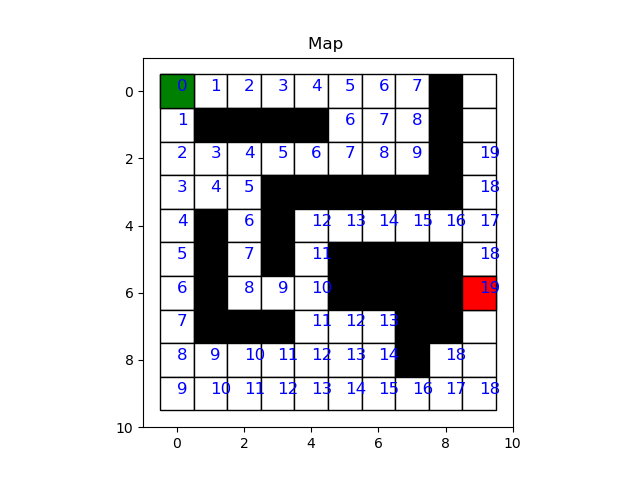
\includegraphics[width=\linewidth]{figures/Dijkstra_Weights.png}
        \label{fig:Dijkstra_Weights_Example}
        \caption{Example of a map populated with the heuristic weights from Dijkstra's Algorithm}
    \end{figure} 

    \section{Breath First Search (BFS)} \label{BFS}
    The main concept behind BFS is that the algorithm explores a graph or map equally in all directions. It is extremely simple and useful, and usually leads to a complete search and an optimal path. However, it takes a long time to compute since there is no heuristic pushing the algorithm to look toward the goal. It is also important to note that BFS algorithms assume there is no difference moving between points on a graph/map - a major limitation especially when path planning.

    \subsection{Implementation}
    BFS is one of the most simple algorithms, usually taking only a few lines of code to fully implement. Below is some basic Python pseudocode describing my implementation of BFS: \cite{RedBlobGames_a*}

    \begin{lstlisting}[language=Python]
frontier = list()
frontier.append(start_node)
visited = dictionary()
visited[start_node] = None

while frontier not empty:
    current = frontier.get_first()
    if goal found in visited:
        exit loop and return path
    for neighbor in neighbors of current:
        if neighbor exists and \
            not in visited and \
            not obstacle:
            frontier.add_to_end(neighbor)
            visited[neighbor] = current
    \end{lstlisting}

    The output of the code above only gives a list of visited nodes and where they were visited from. Therefore, an additional section of code was needed to generate a path:

    \begin{lstlisting} [language=Python]
path = list()
curr_point = goal_node
while curr_point is not start:
        path.append(curr_point)
        curr_point = visited.get(curr_point)
path.append(start)
path.reverse()
    \end{lstlisting}

    Finally, to get the number of steps taken, I simply took the length of the \lstinline{visited} dictionary.

    \subsection{Results}

    \begin{figure}[ht]
        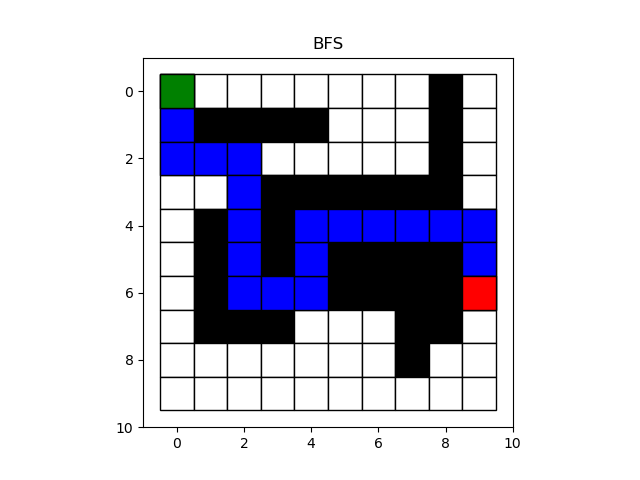
\includegraphics[width=\linewidth]{figures/BFS_LargeMap_Path.png}
        \label{fig:Dijkstra_Weights_Example}
        \caption{Breath First Search Results for a 10x10 map. The algorithm took 64 steps to find the solution.}
    \end{figure} 

    \begin{figure}[ht]
        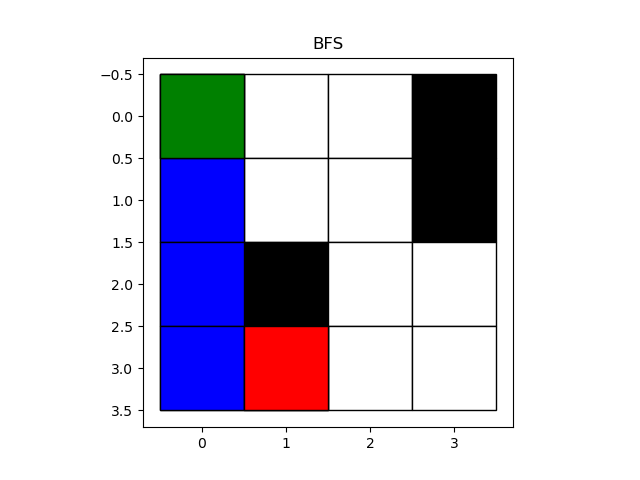
\includegraphics[width=\linewidth]{figures/BFS_SmallMap_Path.png}
        \label{fig:Dijkstra_Weights_Example}
        \caption{Breath First Search result for a 4x4 map. The algorithm took 10 steps to find the solution}
    \end{figure} 

    \section{Depth First Search (DFS)} \label{DFS}

    \subsection{Implementation}
    
    \subsection{Results}

    \begin{figure}[ht]
        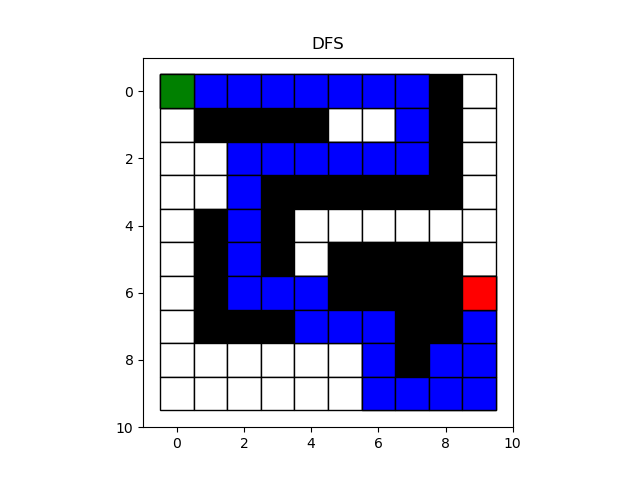
\includegraphics[width=\linewidth]{figures/DFS_LargeMap_Path.png}
        \label{fig:Dijkstra_Weights_Example}
        \caption{Depth First Search result for a 10x10 map. The algorithm took 33 steps to find the solution}
    \end{figure} 

    \begin{figure}[ht]
        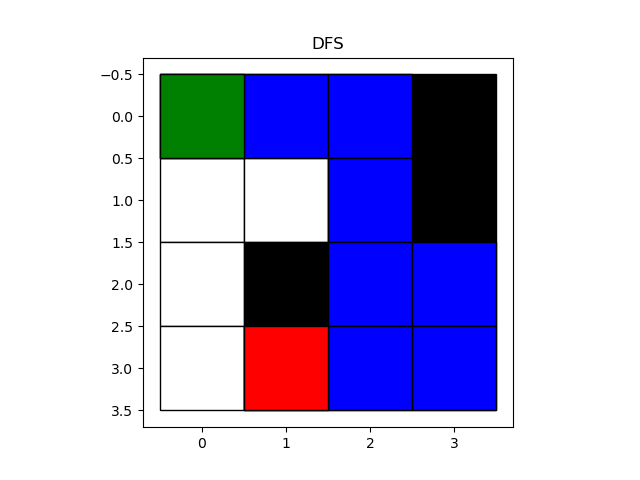
\includegraphics[width=\linewidth]{figures/DFS_SmallMap_Path.png}
        \label{fig:Dijkstra_Weights_Example}
        \caption{Depth First Search result for a 4x4 map. The algorithm took 9 steps to find the solution}
    \end{figure} 

    \section{Dijkstra's Algorithm} \label{Dijkstra}
    Dijkstra's algorithm extends the usefulness Breath First Search by considering path heuristics. This is extremely useful to get a complete and optimal path from a start node to a goal node considering the movement effort going from one node to another. However, like BFS, it takes a very long time since there is no heuristic to push the algorithm to the goal node faster than other methods.

    \subsection{Implementation}
    
    \subsection{Results}

    \begin{figure}[ht]
        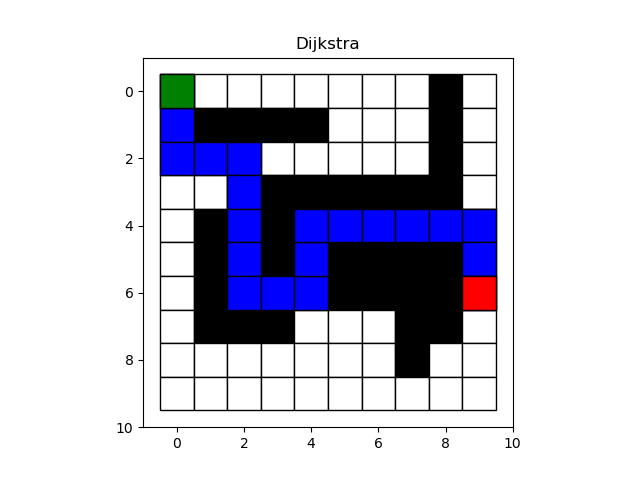
\includegraphics[width=\linewidth]{figures/Dijkstra_LargeMap_Path.png}
        \label{fig:Dijkstra_Weights_Example}
        \caption{Dijkstra's Algorithm search result for a 10x10 map. The algorithm took 64 steps to find the solution}
    \end{figure} 

    \begin{figure}[ht]
        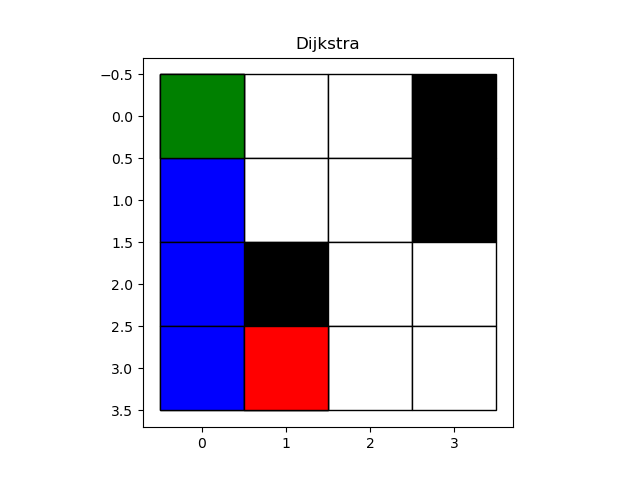
\includegraphics[width=\linewidth]{figures/Dijkstra_SmallMap_Path.png}
        \label{fig:Dijkstra_Weights_Example}
        \caption{Dijkstra's Algorithm search result for a 4x4 map. The algorithm took 10 steps to find the solution}
    \end{figure} 

    \section{A*} \label{A*}

    \subsection{Implementation}
    
    \subsection{Results}

    \begin{figure}[ht]
        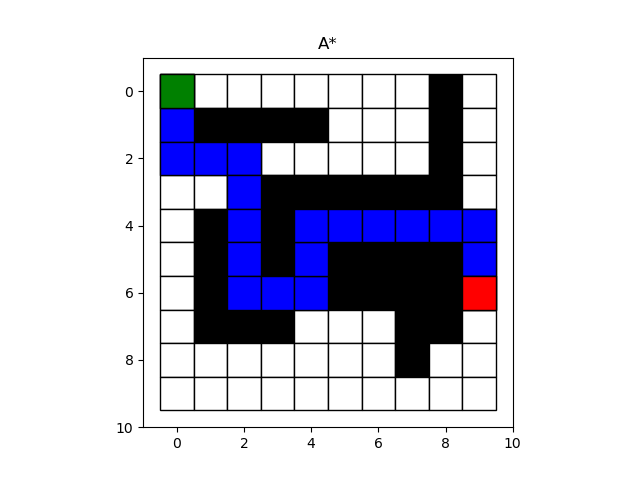
\includegraphics[width=\linewidth]{figures/A_LargeMap_Path.png}
        \label{fig:Dijkstra_Weights_Example}
        \caption{A* search result for a 10x10 map. The algorithm took 48 steps to find the solution}
    \end{figure} 

    \begin{figure}[ht]
        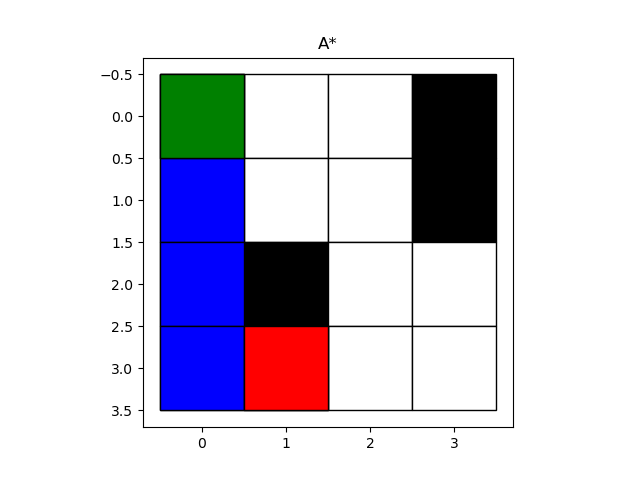
\includegraphics[width=\linewidth]{figures/A_SmallMap_Path.png}
        \label{fig:Dijkstra_Weights_Example}
        \caption{A* search result for a 4x4 map. The algorithm took 8 steps to find the solution}
    \end{figure} 

    \printbibliography

\end{document}